% !TeX root = ../main.tex

\chapter{Evaluation} \label{chapter:evaluation}

This chapter presents the evaluation results of our model on all datasets of chapter \ref{chapter:datasets}. Since the model exhibits a vast number of hyper parameters and each training can take several days, performing an extensive grid search is not possible. That's why we start to explore the model's substantial hyperparameters independently from each other by using the simplest dataset. Afterwards, the acquired knowledge about our model's behavior can then be transferred to the other datasets in order to perform a basic grid search. Beside the quantitative assessment of the model, it is also qualitatively compared to experimental results of related projects at the end of each section.

All experiments are computed on a single Nvidia GeForce GTX Titan X using the TensorFlow open source software library for machine intelligence in version r0.10 with CUDA 7.5.18 and cuDNN 4. This quite new deep learning framework is developed by Google as a second-generation system based on their experiences with DistBelief \parencite{distbelief}. A computation in TensorFlow is expressed as a stateful dataflow graph, where each node represents a mathematical operation and the graph's edges a data tensor that can flow from one node to the next \parencite{tensorflow2015-whitepaper}. It has gained increasing attention since its first public release in November 2015.

If not stated differently, the model configuration described in Chapter \ref{chapter:implementation} is used, but with a two-layer ConvLSTM using $3\times3$ input-to-hidden and $5\times5$ hidden-to-hidden kernel size in the internal convolutions. Further, we deactivate the optional BN-layers within these cells for two reasons. Firstly, first tests have not shown any improvements using them. And secondly, the fact that its TensorFlow implementation back then had the issue\footnote{Further details: \url{https://github.com/tensorflow/tensorflow/issues/4361}} of performing batch statistic updates multiple times when being share across time resulted in an enormous drop in performance. We therefore keep the use of these batch normalizations within the spatio-temporal encoder and decoder components for future work. Additionally, all weights are initialized using the Xavier method of equation \ref{eq:xavier} and the default weight decay regularization coefficient is set to $\lambda=1e^{-5}$. We use a batch size of 32 during the training process together with Adam optimizer ($\beta_1 = 0.9$, $\beta_2 = 0.999$, $\epsilon =1e^{-8}$) and a default initial learning rate of $\eta = 0.001$. In addition to the learning rate annealing mechanism of Adam, the learning rate is also manually decreased once per epoch using a stair-case exponential decay function by a factor of $\alpha=0.9$.

Lastly, it has to be mentioned that diagrams, which show results of any kind of objective function, are always shown with its y-axis in logarithmic scale so that fine differences become better recognizable. And unless otherwise specified, all presented losses can be understood as the average per-pixel error across the whole generated future sequence.

\section{Experiments on Moving MNIST} \label{sec:exp-mm}

The synthetic Moving MNIST dataset is used as a starting point for the evaluation of our model. Given an input sequence of ten frames, the network therefore has to understand and encode the motion of this input in order to predict the next ten frames of the future. In this section, we qualitatively and quantitatively compare our results with other network models, because it has been used in several previous works as well. The loss layer used in this section does not use the SSIM term by default.

\subsection{Model Exploration}

The model is incrementally explored in this section in order to understand its behavior regarding changes in the hyperparameters, as well as to see the effects of the modern techniques used in the training process.

\subsubsection*{Scheduled Sampling}

The consequences of the used scheduled sampling technique are examined first. Figure \ref{fig:plot-mm-asss} visualizes the training and validation binary cross-entropy using our standard model with either scheduled sampling (SS) or always sampling (AS). The latter method means the approach to always sample from the previously generated frame, which is comparable to SS with a constant sampling probability of $p=0$. It can be seen that there is a huge discrepancy between the training and validation error in the starting phase, where the SS-approach mainly trained on input samples taken from the ground truth. The can be explained that sampling on the ground truth in every time step of the recurrent network tremendously speeds up the convergence of the training loss, because each cell does not have to correct errors of the previous cells. In contrary, the validation loss is very bad in this phase, since the results represent the average out of ten predicted frames and the spatio-temporal decoder suddenly receives its own feature space predictions as input to predict the next frame, which is in contrast to the process while training so far.

\begin{figure}[htb]
  \centering
  \pgfplotstableset{col sep=comma}
  \pgfplotstableread{data/mm/as_ss/run_mm-ss-2l3i5hp-c326464k533s212bn-wd1e-05-YT-tag_validation_bce.csv}\modelA
  \pgfplotstableread{data/mm/as_ss/run_mm-as-2l3i5hp-c326464k533s212bn-wd1e-05-SE-tag_validation_bce.csv}\modelB
  \pgfplotstableread{data/mm/as_ss/run_mm-ss-2l3i5hp-c326464k533s212bn-wd1e-05-YT-tag_loss-BCE_loss-Mean.csv}\modelAA
  \pgfplotstableread{data/mm/as_ss/run_mm-as-2l3i5hp-c326464k533s212bn-wd1e-05-SE-tag_loss-BCE_loss-Mean.csv}\modelBB
  \pgfplotstableread{data/mm/as_ss/run_mm-ss-2l3i5hp-c326464k533s212bn-wd1e-05-YT-tag_scheduled_sampling.csv}\modelSS
  \begin{tikzpicture}
    \begin{axis}[
    	axis y line*=right,
    	hide x axis,
    	ylabel near ticks,
        ymin=0,
        ymax=1,
        xmin=0,
        xmax=65000,
        thick,
        ylabel=GT sampling probability \textit{p},
        xlabel=step \textit{i},
        x post scale=1.8,
      ]
      \addplot[draw=LightGoldenrod, thin, opacity=0.8] table[x=Step, y=Value]{\modelSS};\label{mSS}
    \end{axis}
    \begin{axis}[
    	axis y line*=left,
    	ymode=log,
    	log ticks with fixed point,
        ymin=0,
        ymax=0.3,
        xmin=0,
        xmax=65000,
        ytick={0.05,0.075,0.1,0.15,0.2},
        legend style={legend pos=north east},
        grid,
        thick,
        ylabel=BCE loss,
        xlabel=step \textit{i},
        x post scale=1.8,
      ]
	  \addlegendimage{/pgfplots/refstyle=mSS}\addlegendentry{Scheduled Sampling}    
      
      % background
      \addplot[draw=black!10!blue, thin, opacity=0.8] table[x=Step, y=Value]{\modelBB};
      \addlegendentry{AS (train)}
      \addplot[draw=black!10!green, thin, opacity=0.8] table[x=Step, y=Value]{\modelAA};
      \addlegendentry{SS (train)}
      %foreground
      \addplot[draw=black!30!blue] table[x=Step, y=Value]{\modelB};
      \addlegendentry{AS (valid)}
      %best
      \addplot[draw=black!30!green] table[dashed, x=Step, y=Value]{\modelA};
      \addlegendentry{SS (valid)} 
    \end{axis}
    
  \end{tikzpicture}
  \caption[Influences of Scheduled Sampling]{Influences of scheduled sampling regarding the training and validation error in context of recurrent networks and future frames prediction on Moving MNIST.}\label{fig:plot-mm-asss}
\end{figure}

But the interesting insight here is that as soon as the scheduled sampling component completely changed the input behavior to inference mode, the achieved prediction performance is continuously better compared to the approach of always sampling from previous generated frames directly at the very beginning. This behavior could be explained that the SS approach introduces some kind of pre-training phase, where the network can learn to predict the next frame when a perfect current frame is given. Hence, it has not to deal with errors made in the previous time step. By slowly changing this behavior to the mode as it is used while inference, it then also starts to learn a robustness against imperfect input frames. A similar behavior can be seen when comparing the results of the PSNR metric between AA and SS in Figure \ref{fig:plot-mm-asss2-psnr}. However, when we look at the sharpness difference metric in Figure \ref{fig:plot-mm-asss2-sdiffcurve}, it can be seen that sharpness of the predictions is continuously better using scheduled sampling.

\begin{figure}[htb]
\centering
\begin{subfigure}{0.5\textwidth}
  \centering
  \pgfplotstableset{col sep=comma}
  \pgfplotstableread{data/mm/as_ss/run_mm-ss-2l3i5hp-c326464k533s212bn-wd1e-05-YT-tag_validation_sharpdiff.csv}\modelA
  \pgfplotstableread{data/mm/as_ss/run_mm-as-2l3i5hp-c326464k533s212bn-wd1e-05-SE-tag_validation_sharpdiff.csv}\modelB
  \hspace*{-0.6cm}
  {
  \begin{tikzpicture}[scale=0.5]
    \begin{axis}[
        ymin=10,
        ymax=15,
        xmin=0,
        xmax=65000,
        legend style={legend pos=south east},
        grid,
        thick,
        ylabel=SharpDiff,
        xlabel=step \textit{i},
        x post scale=1.6,
      ]
      \addplot[draw=black!30!blue] table[x=Step, y=Value]{\modelB};
      \addlegendentry{AS (valid)};
      %best
      \addplot[draw=black!30!green] table[x=Step, y=Value]{\modelA};
      \addlegendentry{SS (valid)};
    \end{axis}
  \end{tikzpicture}
  }
  \caption{}
  \label{fig:plot-mm-asss2-sdiffcurve}
\end{subfigure}%
\begin{subfigure}{0.5\textwidth}
  \centering
  \pgfplotstableset{col sep=comma}
  \pgfplotstableread{data/mm/as_ss/run_mm-ss-2l3i5hp-c326464k533s212bn-wd1e-05-YT-tag_validation_psnr.csv}\modelA
  \pgfplotstableread{data/mm/as_ss/run_mm-as-2l3i5hp-c326464k533s212bn-wd1e-05-SE-tag_validation_psnr.csv}\modelB
  \hspace*{-0.6cm}
  {
  \begin{tikzpicture}[scale=0.5]
    \begin{axis}[
        ymin=10,
        ymax=20,
        xmin=0,
        xmax=65000,
        legend style={legend pos=south east},
        grid,
        thick,
        ylabel=PSNR,
        xlabel=step \textit{i},
        x post scale=1.6,
      ]
      \addplot[draw=black!30!blue] table[x=Step, y=Value]{\modelB};
      \addlegendentry{AS (valid)};
      %best
      \addplot[draw=black!30!green] table[x=Step, y=Value]{\modelA};
      \addlegendentry{SS (valid)};
    \end{axis}
  \end{tikzpicture}
  }
  \caption{}
  \label{fig:plot-mm-asss2-psnr}
\end{subfigure}
\caption[Image Metrics Comparing AS and SS]{Comparison of validation results based on a model with either using the scheduled sampling or the always sampling training technique.} \label{fig:plot-mm-asss2}
\end{figure}



\subsubsection*{Batch Normalization}

The use of batch normalization in the spatial encoder and decoder components is investigated next. Figure \ref{fig:plot-mm-bn} shows a clear advantage of using BN-layers. It can be argued that our model is able to profit strongly from batch normalization, because it does not only support the convolutional encoder and decoder to learn faster by compensating the internal covariate shift. Also, both recurrent networks in-between can benefit from this, reasoned by the fact that the frame representations in feature space, that are produced by the spatial encoders, tend to have a more stable distribution. Consequently, the spatio-temporal encoder has fewer problems to extract useful patterns from these representations while consuming them in the course of the training process.

\begin{figure}[htb]
\centering
\begin{subfigure}{0.5\textwidth}
  \centering
  \pgfplotstableset{col sep=comma}
  \pgfplotstableread{data/mm/bn/run_mm-ss-2l3i5hp-c326464k533s212bn-wd1e-05-XG-tag_validation_bce.csv}\modelA
  \pgfplotstableread{data/mm/bn/run_mm-ss-2l3i5hp-c326464k533s212-wd1e-05-MX-tag_validation_bce.csv}\modelB
  \hspace*{-0.6cm}
  {
  \begin{tikzpicture}[scale=0.5]
    \begin{axis}[
        ymode=log,
    	log ticks with fixed point,
        ymin=0,
        ymax=0.3,
        xmin=0,
        xmax=65000,
        legend style={legend pos=north east},
        grid,
        thick,
        ylabel=BCE loss,
        xlabel=step \textit{i},
        x post scale=1.6,
      ]
      \addplot[draw=black!30!blue] table[x=Step, y=Value]{\modelB};
      \addlegendentry{w/o BN (valid)};
      %best
      \addplot[draw=black!30!green] table[x=Step, y=Value]{\modelA};
      \addlegendentry{with BN (valid)};
    \end{axis}
  \end{tikzpicture}
  }
  \caption{}
  \label{fig:plot-mm-bn-bce}
\end{subfigure}%
\begin{subfigure}{0.5\textwidth}
  \centering
  \pgfplotstableset{col sep=comma}
  \pgfplotstableread{data/mm/bn/run_mm-ss-2l3i5hp-c326464k533s212bn-wd1e-05-XG-tag_validation_sharpdiff.csv}\modelA
  \pgfplotstableread{data/mm/bn/run_mm-ss-2l3i5hp-c326464k533s212-wd1e-05-MX-tag_validation_sharpdiff.csv}\modelB
  \hspace*{-0.6cm}
  {
  \begin{tikzpicture}[scale=0.5]
    \begin{axis}[
        ymin=10,
        ymax=15,
        xmin=0,
        xmax=65000,
        legend style={legend pos=south east},
        grid,
        thick,
        ylabel=SharpDiff,
        xlabel=step \textit{i},
        x post scale=1.6,
      ]
      \addplot[draw=black!30!blue] table[x=Step, y=Value]{\modelB};
      \addlegendentry{w/o BN (valid)};
      %best
      \addplot[draw=black!30!green] table[x=Step, y=Value]{\modelA};
      \addlegendentry{with BN (valid)};
    \end{axis}
  \end{tikzpicture}
  }
  \caption{}
  \label{fig:plot-mm-bn-psnr}
\end{subfigure}
\caption[Influences of Batch Normalization]{Comparison of the validation results from two model instances where one uses batch normalization layers in the spatial encoder and decoder components.} \label{fig:plot-mm-bn}
\end{figure}


\subsubsection*{Learning Rate Decay}

The network's learning behavior using two different exponential decay rates is illustrated in Figure \ref{fig:plot-mm-lr}. In this example, the learning rate is slightly decayed after each epoch by a specified factor. Because the Moving MNIST dataset is generated on-the-fly, we specify its total size to be virtually \num{32000}. In this way, the learning rate is effectively decayed after each validation step\footnote{In the course of this evaluation, we assess our model in a full epoch on the validation set every \nth{1000} training step.}, since a batch size of \num{32} is used. The network denoted with blue has a clear disadvantage, because its learning rate at the end became so small that it almost stops learning. However, throughout our experiments we determined that a very low learning rate at the end of the training was beneficial regarding the image quality and finer details of the generated images.

\begin{figure}[htb]
  \centering
  \pgfplotstableset{col sep=comma}
  \pgfplotstableread{data/mm/lr/run_mm-ss-2l3i5hp-c326464k533s212bn-wd1e-05-JK-tag_validation_bce.csv}\modelA
  \pgfplotstableread{data/mm/lr/run_mm-ss-2l3i5hp-c326464k533s212bn-wd1e-05-XG-tag_validation_bce.csv}\modelB
  \pgfplotstableread{data/mm/lr/run_mm-ss-2l3i5hp-c326464k533s212bn-wd1e-05-JK-tag_learning_rate.csv}\modelLrA
  \pgfplotstableread{data/mm/lr/run_mm-ss-2l3i5hp-c326464k533s212bn-wd1e-05-XG-tag_learning_rate.csv}\modelLrB
  \begin{tikzpicture}
    \begin{axis}[
    	axis y line*=right,
    	hide x axis,
    	ylabel near ticks,
        ymin=0,
        ymax=0.001,
        xmin=0,
        xmax=65000,
        thick,
        ylabel={Learning rate $\eta$},
        xlabel=step \textit{i},
        x post scale=1.8,
      ]
      \addplot[draw=black!10!blue, very thin, opacity=0.8] table[x=Step, y=Value]{\modelLrB};\label{mB}
      \addplot[draw=black!10!green, very thin, opacity=0.8] table[x=Step, y=Value]{\modelLrA};\label{mA}
    \end{axis}
    \begin{axis}[
    	axis y line*=left,
    	ymode=log,
    	log ticks with fixed point,
        ymin=0,
        ymax=0.3,
        xmin=0,
        xmax=65000,
        ytick={0.05,0.075,0.1,0.15,0.2},
        legend style={legend pos=north east},
        grid,
        thick,
        ylabel=BCE loss,
        xlabel=step \textit{i},
        x post scale=1.8,
      ]
	  \addlegendimage{/pgfplots/refstyle=mB}\addlegendentry{$\eta$-decay=0.90 (valid)}
      \addlegendimage{/pgfplots/refstyle=mA}\addlegendentry{$\eta$-decay=0.95 (valid)}
      
      %foreground
      \addplot[draw=black!30!blue] table[x=Step, y=Value]{\modelB};
      \addlegendentry{$\eta$-decay=0.90};
      %best
      \addplot[draw=black!30!green] table[dashed, x=Step, y=Value]{\modelA};
      \addlegendentry{$\eta$-decay=0.90};
    \end{axis}
  \end{tikzpicture}
  \caption[Influences of Learning Rate Decay]{Validation losses of two identical network models using different learning rate decay rates in combination with Adam optimizer.}\label{fig:plot-mm-lr}
\end{figure}


\subsubsection*{ConvLSTM Feature Maps}

Next, we investigate the network's behavior with respect to the hidden-to-hidden feature maps in the spatio-temporal decoder and encoder components. Therefore, we adjust the number of feature maps produced by the convolutional layers in the spatial encoder. While a simpler variant is used that produces (16, 32, 32) feature maps in each layer at first, another more complex variant is used as well which convolves (64, 128, 128) feature maps. The number feature maps produced by the last layer is then used constantly within the ConvLSTM cells and its temporal transitions. Consequently, the performance of these two model configurations is compared against the standard model with 64 temporal feature maps in Figure \ref{fig:plot-mm-filter}.

\begin{figure}[htb]
\centering
\begin{subfigure}{0.5\textwidth}
  \centering
  \pgfplotstableset{col sep=comma}
  \pgfplotstableread{data/mm/filters/run_mm-ss-2l3i5hp-c326464k533s212bn-wd1e-04-FG-tag_validation_bce.csv}\modelA
  \pgfplotstableread{data/mm/filters/run_mm-ss-2l3i5hp-c163232k533s212bn-wd1e-04-YP-tag_validation_bce.csv}\modelB
  \pgfplotstableread{data/mm/filters/run_mm-ss-2l3i5hp-c64128128k533s212bn-wd1e-05-NK-tag_validation_bce.csv}\modelC
  \hspace*{-0.6cm}
  {
  \begin{tikzpicture}[scale=0.5]
    \begin{axis}[
        ymode=log,
    	log ticks with fixed point,
        ymin=0,
        ymax=0.3,
        xmin=0,
        xmax=65000,
        ytick={0.05,0.075,0.1,0.15,0.2},
        legend style={legend pos=north east},
        grid,
        thick,
        ylabel=BCE loss,
        xlabel=step \textit{i},
        x post scale=1.6,
      ]
      \addplot[draw=black!30!blue] table[x=Step, y=Value]{\modelB};
      \addlegendentry{32 feature maps (valid)};
      %best
      \addplot[draw=black!30!green] table[x=Step, y=Value]{\modelA};
      \addlegendentry{64 feature maps (valid)};
      
      \addplot[draw=black!30!red] table[x=Step, y=Value]{\modelC};
      \addlegendentry{128 feature maps (valid)};
    \end{axis}
  \end{tikzpicture}
  }
  \caption{}
  \label{fig:plot-mm-filter-bce}
\end{subfigure}%
\begin{subfigure}{0.5\textwidth}
  \centering
  \pgfplotstableset{col sep=comma}
  \pgfplotstableread{data/mm/filters/run_mm-ss-2l3i5hp-c326464k533s212bn-wd1e-04-FG-tag_validation_ssim.csv}\modelA
  \pgfplotstableread{data/mm/filters/run_mm-ss-2l3i5hp-c163232k533s212bn-wd1e-04-YP-tag_validation_ssim.csv}\modelB
  \pgfplotstableread{data/mm/filters/run_mm-ss-2l3i5hp-c64128128k533s212bn-wd1e-05-NK-tag_validation_ssim.csv}\modelC
  \hspace*{-0.6cm}
  {
  \begin{tikzpicture}[scale=0.5]
    \begin{axis}[
        ymin=0.5,
        ymax=1.0,
        xmin=0,
        xmax=65000,
        legend style={legend pos=south east},
        grid,
        thick,
        ylabel=SSIM,
        xlabel=step \textit{i},
        x post scale=1.6,
      ]
      \addplot[draw=black!30!blue] table[x=Step, y=Value]{\modelB};
      \addlegendentry{32 feature maps};
      %best
      \addplot[draw=black!30!green] table[x=Step, y=Value]{\modelA};
      \addlegendentry{64 feature maps};
      
      \addplot[draw=black!30!red] table[x=Step, y=Value]{\modelC};
      \addlegendentry{128 feature maps};
    \end{axis}
  \end{tikzpicture}
  }
  \caption{}
  \label{fig:plot-mm-filter-psnr}
\end{subfigure}
\caption[Influences of ConvLSTM Feature Maps]{Impact of the number of feature maps within the ConvLSTM encoder and decoder networks regarding overall frame prediction performance.} \label{fig:plot-mm-filter}
\end{figure}

As expected, the network with only 32 feature maps performs worse compared to the standard setting. But it is very surprising that the model configuration with 128 feature maps achieves even worse results. One possible reason could be an unfavorable, random initialization of the initial model parameters. However, due to the fact that such a network configuration requires roughly the entire video memory of the GPU, as well as takes twice as long to train, we came to the decision to continue our experiments on 64 feature maps only.


\subsubsection*{ConvLSTM Layers}

The number of recurrent layers has a very positive effect in order to generate future frames of better quality. The same behavior has also been mentioned in the practical experiment of \parencite[p. 6]{unsup_learn_lstm}, where they have qualitatively shown that a deeper LSTM is able to generate sharper images. Figure \ref{fig:plot-mm-layer} shows that the improvements of adding a third layer is apparently smaller compared to the difference when a second layer is added. Unfortunately, a 4-layer network could not be tested due to memory limitations of the graphics card. Additionally, it is worthwhile noting that the number of recurrent layers has a huge impact in respect to model complexity, training time and memory requirements.

\begin{figure}[htb] % note: these use triplet loss already!!!
\centering
\begin{subfigure}{0.5\textwidth}
  \centering
  \pgfplotstableset{col sep=comma}
  \pgfplotstableread{data/mm/layers/run_mm-ss-3l3i5hp-c326464k533s212bn-wd1e-05-triplet-JM-tag_validation_bce.csv}\modelA
  \pgfplotstableread{data/mm/layers/run_mm-ss-2l3i5hp-c326464k533s212bn-wd1e-05-triplet-CE-tag_validation_bce.csv}\modelB
  \pgfplotstableread{data/mm/layers/run_mm-ss-1l3i5hp-c326464k533s212bn-wd1e-05-triplet-MK-tag_validation_bce.csv}\modelC
  \hspace*{-0.6cm}
  {
  \begin{tikzpicture}[scale=0.5]
    \begin{axis}[
    	ymode=log,
    	log ticks with fixed point,
        ymin=0,
        ymax=0.3,
        xmin=0,
        xmax=65000,
        ytick={0.05,0.075,0.1,0.15,0.2},
        legend style={legend pos=north east},
        grid,
        thick,
        ylabel=BCE loss,
        xlabel=step \textit{i},
        x post scale=1.6,
      ]
      \addplot[draw=black!30!red] table[x=Step, y=Value]{\modelC};
      \addlegendentry{1-layer ConvLSTM};
      \addplot[draw=black!30!blue] table[x=Step, y=Value]{\modelB};
      \addlegendentry{2-layer ConvLSTM};
      %best
      \addplot[draw=black!30!green] table[x=Step, y=Value]{\modelA};
      \addlegendentry{3-layer ConvLSTM};
    \end{axis}
  \end{tikzpicture}
  }
  \caption{}
  \label{fig:plot-mm-layer-bce}
\end{subfigure}%
\begin{subfigure}{0.5\textwidth}
  \centering
  \pgfplotstableset{col sep=comma}
  \pgfplotstableread{data/mm/layers/run_mm-ss-3l3i5hp-c326464k533s212bn-wd1e-05-triplet-JM-tag_validation_psnr.csv}\modelA
  \pgfplotstableread{data/mm/layers/run_mm-ss-2l3i5hp-c326464k533s212bn-wd1e-05-triplet-CE-tag_validation_psnr.csv}\modelB
  \pgfplotstableread{data/mm/layers/run_mm-ss-1l3i5hp-c326464k533s212bn-wd1e-05-triplet-MK-tag_validation_psnr.csv}\modelC
  \hspace*{-0.6cm}
  {
  \begin{tikzpicture}[scale=0.5]
    \begin{axis}[
        ymin=10,
        ymax=20,
        xmin=0,
        xmax=65000,
        legend style={legend pos=south east},
        grid,
        thick,
        ylabel=PSNR,
        xlabel=step \textit{i},
        x post scale=1.6,
      ]
      \addplot[draw=black!30!red] table[x=Step, y=Value]{\modelC};
      \addlegendentry{1-layer ConvLSTM};
      \addplot[draw=black!30!blue] table[x=Step, y=Value]{\modelB};
      \addlegendentry{2-layer ConvLSTM};
      %best
      \addplot[draw=black!30!green] table[x=Step, y=Value]{\modelA};
      \addlegendentry{3-layer ConvLSTM};
    \end{axis}
  \end{tikzpicture}
  }
  \caption{}
  \label{fig:plot-mm-layer-psnr}
\end{subfigure}
\caption[Influences of ConvLSTM Layers]{Validation performance of network models with a varying number of recurrent layers. All three models are trained using the triplet loss function.} \label{fig:plot-mm-layer}
\end{figure}



\subsubsection*{Loss Layer}

As a last experiment of our test series, we examine the impact of the different loss terms. Three networks with the identical standard configurations, but different objective functions have therefore been trained. Starting from a network using binary cross-entropy only, perceptual motivated loss terms like GDL and SSIM are added one after another until we end up in the triplet loss described in equation \ref{eq:triplet}. The validation results are depicted in Figure \ref{fig:plot-mm-loss}.

\begin{figure}[htb]
\centering
\begin{subfigure}{0.5\textwidth}
  \centering
  \pgfplotstableset{col sep=comma}
  \pgfplotstableread{data/mm/loss/run_mm-ss-2l3i5hp-c326464k533s212bn-wd1e-05-mae_only-HE,tag_validation_bce.csv}\modelA
  \pgfplotstableread{data/mm/loss/run_mm-ss-2l3i5hp-c326464k533s212bn-wd1e-05-JK,tag_validation_bce.csv}\modelB
  \pgfplotstableread{data/mm/loss/run_mm-ss-2l3i5hp-c326464k533s212bn-wd1e-05-triplet-CE,tag_validation_bce.csv}\modelC
  \hspace*{-0.6cm}
  {
  \begin{tikzpicture}[scale=0.5]
    \begin{axis}[
        ymode=log,
    	log ticks with fixed point,
        ymin=0,
        ymax=0.3,
        xmin=0,
        xmax=65000,
        legend style={legend pos=north east},
        grid,
        thick,
        ylabel=BCE loss,
        xlabel=step \textit{i},
        x post scale=1.6,
      ]
      \addplot[draw=black!30!red] table[x=Step, y=Value]{\modelC};
      \addlegendentry{BCE+GDL+SSIM (valid)};
      \addplot[draw=black!30!blue] table[x=Step, y=Value]{\modelB};
      \addlegendentry{BCE+GDL (valid)};
      %best
      \addplot[draw=black!30!green] table[x=Step, y=Value]{\modelA};
      \addlegendentry{BCE (valid)};
    \end{axis}
  \end{tikzpicture}
  }
  \caption{}
  \label{fig:plot-mm-loss-bce}
\end{subfigure}%
\begin{subfigure}{0.5\textwidth}
  \centering
  \pgfplotstableset{col sep=comma}
  \pgfplotstableread{data/mm/loss/run_mm-ss-2l3i5hp-c326464k533s212bn-wd1e-05-mae_only-HE,tag_validation_sharpdiff.csv}\modelA
  \pgfplotstableread{data/mm/loss/run_mm-ss-2l3i5hp-c326464k533s212bn-wd1e-05-JK,tag_validation_sharpdiff.csv}\modelB
  \pgfplotstableread{data/mm/loss/run_mm-ss-2l3i5hp-c326464k533s212bn-wd1e-05-triplet-CE,tag_validation_sharpdiff.csv}\modelC
  \hspace*{-0.6cm}
  {
  \begin{tikzpicture}[scale=0.5]
    \begin{axis}[
        ymin=10,
        ymax=15,
        xmin=0,
        xmax=65000,
        legend style={legend pos=south east},
        grid,
        thick,
        ylabel=SharpDiff,
        xlabel=step \textit{i},
        x post scale=1.6,
      ]
      \addplot[draw=black!30!red] table[x=Step, y=Value]{\modelC};
      \addlegendentry{BCE+GDL+SSIM (valid)};
      \addplot[draw=black!30!blue] table[x=Step, y=Value]{\modelB};
      \addlegendentry{BCE+GDL (valid)};
      %best
      \addplot[draw=black!30!green] table[x=Step, y=Value]{\modelA};
      \addlegendentry{BCE (valid)};
    \end{axis}
  \end{tikzpicture}
  }
  \caption{}
  \label{fig:plot-mm-loss-psnr}
\end{subfigure}
\caption[Influences of the Loss Term]{Comparison of the validation loss using different objective functions.} \label{fig:plot-mm-loss}
\end{figure}

While the network purely trained on the BCE loss function performs best regarding the binary cross-entropy on the validation set, it nevertheless performs worst according to the sharpness difference metric shown in Figure \ref{fig:plot-mm-loss-psnr}. These results are not surprising, because network using the triplet loss function for example is putting more emphasis on other properties, in contrast to specifically optimizing it regarding to the binary cross-entropy. However, after we have qualitatively analyzed many generated prediction samples in the course of our experiments, we had the impression that results using the simple BCE loss produced the best results. Especially in samples where one handwritten number crosses the other number, the predictions multiple time steps afterwards kept slightly more stable. All in all, perceptual motivated loss terms seem to be useless or even slightly counter-productive when applied on binary Moving MNIST image frames. 

\subsection{Test Results}

For the final evaluation of our model with Moving MNIST, we assess the qualitative and quantitative performance of the best configuration on the test set. Inspired by the findings of our model exploration, as well a rudimentary grid-search, the model for this final test ends up to use the default settings as described earlier, but with an exponential learning rate decay of $\alpha=0.95$ and a loss layer that utilizes no perceptual motivated loss term. We have trained three models of this network with different numbers of recurrent layers for \num{100000} steps.


\subsubsection{Quantitative Results}

A comparison of our best performing model with experimental results of other works is given in Table \ref{tab:mm-comparison}. It can be seen that our model exhibits way less model parameters, especially compared to FC-LSTM approaches. Nevertheless, our ConvLSTM model is able to cut the average pixel-wise test error of the best performing competitive model in halves. The listed results are taken from several published papers. However, we were not able to reproduce the results of FC-LSTM-Combo published in \parencite{unsup_learn_lstm} using their open-source code. After training the model for about \num{1000000} training steps, which took almost one week, the results were not nearly as good as in the paper. Even about \num{20000} training iterations are already sufficient for our model to generate better results.

\begin{table}[htb]
  \small
  \centering
  \begin{tabular}{l r r}
    \toprule
      \textbf{Model} & \textbf{Trainable parameters} & \textbf{BCE test error} \\
    \midrule
      FC-LSTM-Combo(2048-2048) \tiny{\parencite{unsup_learn_lstm}} & \num{214001664} & 0.0855 \\
      FC-LSTM(2048-2048) \tiny{\parencite{conv_lstm_nowcasting}} & \num{142667776} & 0.1180 \\
      ConvLSTM(5/128-64-64) \tiny{\parencite{conv_lstm_nowcasting}} & \num{7585296} & 0.0896 \\
      2enc-ConvLSTM(7/45-45)\footnote{Single frame prediction result, not the average error ofall 10 predicted future frames.} \tiny{\parencite{spat_temp_video_autoenc}} & \num{6132203} & 0.0835 \\
    \midrule
      3enc-ConvLSTM-SS-3dec(5/64) & \num{1841793} & 0.0524 \\
      3enc-ConvLSTM-SS-3dec(5/64-64) & \num{3570817} & 0.0414 \\
      3enc-ConvLSTM-SS-3dec(5/64-64-64) & \num{5299841} & \textbf{0.0407} \\
    \bottomrule
  \end{tabular}
  \caption[Results on Moving MNIST]{Comparison with other networks on Moving MNIST. The numbers in brackets identify the \textit{amount of hidden units} per layer in case of FC-LSTMs, and for ConvLSTMs the \textit{hidden-to-hidden kernel size} followed by the \textit{feature maps per layer} are listed. Further, \textit{3enc} denotes tree convolutional layers in the spatial encoder. We call our model 3enc-ConvLSTM-SS-3dec.}\label{tab:mm-comparison}
\end{table}

\subsubsection{Qualitative Results}

Next, several future frame prediction samples are qualitatively compared with results of other models presented earlier in chapter \ref{chapter:relatedwork}. To that end, we take all Moving MNIST examples that are published in other works and apply our network on exactly the same input data. The contrast against an FC-LSTM approach can be seen in Figures \ref{fig:mm-pred-spec-lstm1} or \ref{fig:mm-pred-spec-lstm1}, as well as the comparison with another ConvLSTM implementation in Figure \ref{fig:mm-pred-spec2-clstm1}. The outcomes of our two-layer model are slightly sharper and much brighter in all three examples. However, the digits \num{3} and \num{0} in Figure \ref{fig:mm-pred-spec-lstm} show some visible artifacts at the end of the predicted future sequence.

\begin{figure}[h!tb]
\centering
\begin{subfigure}{0.49\textwidth}
  \centering
  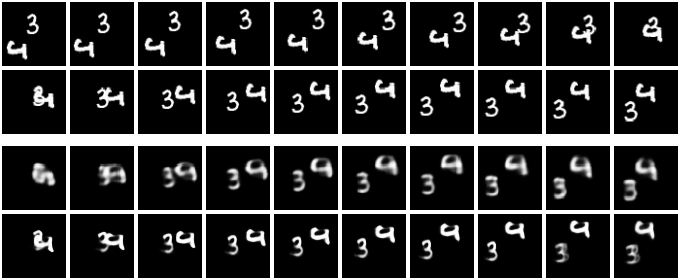
\includegraphics[width=0.92\linewidth]{figures/pred/mm/spec/prediction-00.png}
  \caption{}
  \label{fig:mm-pred-spec-lstm1}
\end{subfigure}%
\begin{subfigure}{0.49\textwidth}
  \centering
  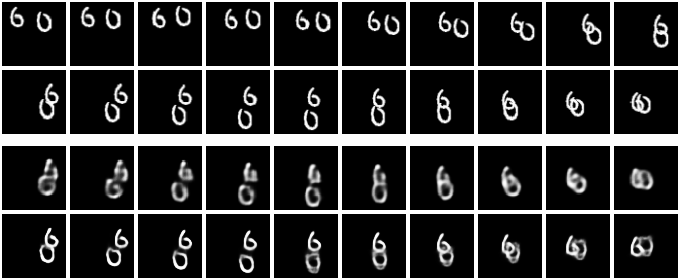
\includegraphics[width=0.92\linewidth]{figures/pred/mm/spec/prediction-01.png}
  \caption{}
  \label{fig:mm-pred-spec-lstm2}
\end{subfigure}
\begin{subfigure}{0.49\textwidth}
  \centering
  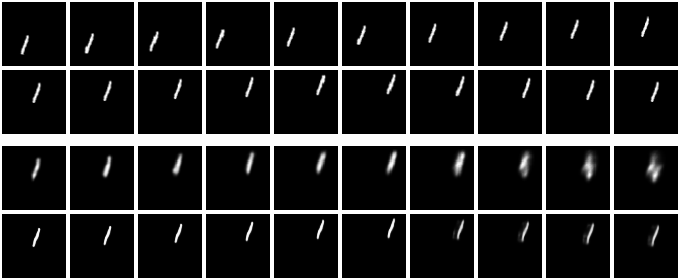
\includegraphics[width=0.92\linewidth]{figures/pred/mm/spec/prediction-02.png}
  \caption{}
  \label{fig:mm-pred-spec-lstm3}
\end{subfigure}
\begin{subfigure}{0.49\textwidth}
  \centering
  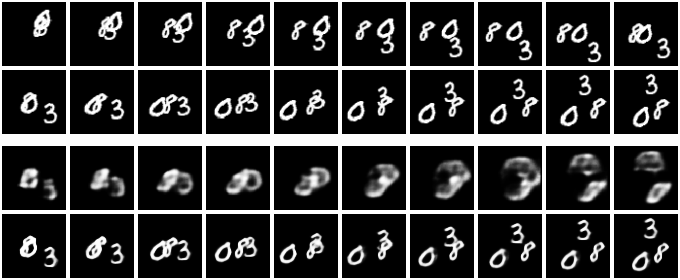
\includegraphics[width=0.92\linewidth]{figures/pred/mm/spec/prediction-03.png}
  \caption{}
  \label{fig:mm-pred-spec-lstm4}
\end{subfigure}
\caption[Comparison with LSTM on Moving MNIST]{Qualitative comparison with FC-LSTM-Combo(2048-2048) \parencite{unsup_learn_lstm}. Experiments in (c) and (d) are using a different number of digits than the network was trained for. From top to bottom: inputs sequence; ground truth target sequence; predictions of FC-LSTM-Combo; predictions of our 2-layer model.} \label{fig:mm-pred-spec-lstm}
\end{figure}

Further predictions of our model, which have been randomly chosen from the Moving MNIST test set, can be found in Figure \ref{fig:mm-pred-random} in the appendix. While most generated results look quite similar to the ground truth future, the sample in Figure \ref{fig:mm-pred-random2} clearly shows that the model still has its issues to preserve details when both digits overlap each other over a longer period.


\subsubsection{Out-of-Domain Results}

Additionally, we verify the model's ability to deal with data that is outside the domain it has been trained for. We therefore take several Moving MNIST sequences that use one or three digits instead of two and compare the generated results with predictions generated by other competitive models. At this point, it is to highlight that we are not just cherry-picking the best generated predictions in this experiment, because we take the exact same sequences that have been used in related works. In a manner of speaking, we are probably using input sequences where other network models have performed best.

\begin{figure}[h!tb]
\centering
\begin{subfigure}{0.49\textwidth}
  \centering
  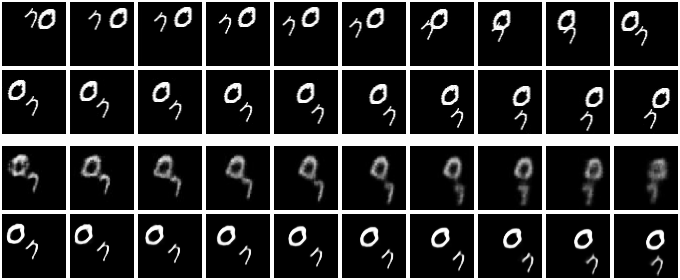
\includegraphics[width=0.92\linewidth]{figures/pred/mm/spec/prediction-04.png}
  \caption{}
  \label{fig:mm-pred-spec2-clstm1}
\end{subfigure}%
\begin{subfigure}{0.49\textwidth}
  \centering
  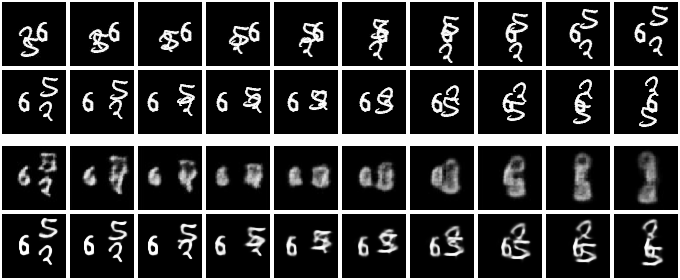
\includegraphics[width=0.92\linewidth]{figures/pred/mm/spec/prediction-05.png}
  \caption{}
  \label{fig:mm-pred-spec2-clstm2}
\end{subfigure}
\caption[Comparison with other ConvLSTM on Moving MNIST]{Qualitative comparison with ConvLSTM(5/128-64-64 \parencite{conv_lstm_nowcasting}. The experiment in (b) uses more digits than the network was trained for. From top to bottom: inputs sequence; ground truth target sequence; prediction results of the competitive model; predictions of our 2-layer ConvLSTM.} \label{fig:mm-pred-spec2-clstm}
\end{figure}

A remarkable difference is visible when the outcomes of our model is qualitatively compared with predictions of existing approaches. In case of the samples using three digits in Figures \ref{fig:mm-pred-spec-lstm4} and \ref{fig:mm-pred-spec2-clstm2}, the structure of each digit stays more stable and does not get washed-out, even after a digit has been overlapped by both others. Moreover, it does not try to merge two numbers in order to end up with the same number of digits like the networks have been trained for. A similar behavior can be seen in Figure \ref{fig:mm-pred-spec-lstm3}, where only a single digit is used. In that scenario, the other network model clearly tries to hallucinate a second flying number at the end of the future sequence. This misbehavior is not visible in the outputs of our model.

Further out-of-domain results can be found in Figure \ref{fig:mm-pred-long} in the appendix. It shows the scenario where our model tries to predict a much longer sequence than it has been trained for. Such a scenario is very to realize with our model due to its recurrent encoder-decoder architecture. We therefore unroll the spatio-temporal decoder component for \num{30} time steps in order to verify the long-term stability of the predicted frames. It can be seen that the network is able to continuously produce acceptable results, with the exception of the last five frame in Figure \ref{fig:mm-pred-long1}. From about the \nth{30} predicted future frame, our model then starts to produce very noisy outcomes in almost every case.






























\section{Experiments on MsPacman} \label{sec:exp-pac}

The network model is applied on the MsPacman dataset in our second experiment to see how it behaves with data of increased complexity. The effects of perceptual motivated loss terms are investigated more deeply in this dataset, because we strongly belief that their weaknesses in Section \ref{sec:exp-mm} are cause by the unnaturally of binary image data.


\subsection{Hyperparameter Tuning} \label{sec:hyper_pac}

In order to find good hyperparameters for the network model, we started to use the best performing model of Moving MNIST, but with the four modifications. First, the three layers of the spatial encoder and decoder components are using strides of $s_i=(1, 2, 1)$ instead $s_i=(2, 1, 2)$, where $i$ denotes the index of the convolutional layer, in order to end up with a feature space representation of the same shape as before. This change is caused by the fact that the model is trained on smaller $32 \times 32$ patches. Second, we use a \textit{tanh} activation function in the output layer so that each generated frame is within the valid scale. Third, a learning rate decay of $\alpha=0.95$ per epoch is used by default. And lastly, the triplet loss function of Section \ref{sec:impl-components} with MAE as the main loss function is used as a starting point in this evaluation, because previous works have shown its advantages in image processing tasks compared to squared error.

We trained several networks with different numbers of recurrent layers, varying initial learning rates $\eta \in \{0.0005, 0.001, 0.005\}$, as well as different weight decays $\lambda \in \{1e^{-6}, 1e^{-5}, 1e^{-4}\} $. While we could see a clear improvement between the single layer and two-layer ConvLSTM model, there has been no clear benefit from using a third layer. The differences in results when we performed variations in learning rate and weight decay have also been marginal. Eventually, we ended up with an initial learning rate of $\eta = 0.0005 $ and continued to use the default weight decay of $\lambda = 1e^{-5}$. Further, we used the two-layer model with the main reason to save training time.


\subsubsection*{Loss Layer}

Even that we couldn't improve our network's performance by performing variations in several hyperparameters that much, we experienced that variations in the objective function could cause more noticeable differences in both quantitative and qualitative results. As a consequence, we decided to do a further investigation by using different loss terms. Several validation results are therefore illustrated in Figure \ref{fig:plot-pac-loss}. 

\begin{figure}[htb]
\centering
\begin{subfigure}{0.5\textwidth}
  \centering
  \pgfplotstableset{col sep=comma}
  \pgfplotstableread{data/pac/loss/mse/run_pac-ss-2l3i5hp-c326464k533s121bn-wd1e-05-mse-triplet-MZ_validation_mse.csv}\modelA
  \pgfplotstableread{data/pac/loss/mse/run_pac-ss-2l3i5hp-c326464k533s121bn-wd1e-05-mse-QQ_validation_mse.csv}\modelB
  \pgfplotstableread{data/pac/loss/mse/run_pac-ss-2l3i5hp-c326464k533s121bn-wd1e-05-mae-triplet-VY_validation_mse.csv}\modelC
  \pgfplotstableread{data/pac/loss/mse/run_pac-ss-2l3i5hp-c326464k533s121bn-wd1e-05-mae-LU_validation_mse.csv}\modelD
  \hspace*{-0.6cm}
  {
  \begin{tikzpicture}[scale=0.5]
    \begin{axis}[
        ymode=log,
    	log ticks with fixed point,
        ymin=0,
        ymax=0.3,
        xmin=0,
        xmax=100000,
        legend style={legend pos=north east},
        grid,
        thick,
        ylabel=MSE loss,
        xlabel=step \textit{i},
        x post scale=1.6,
      ]
      \addplot[draw=black!30!orange] table[x=Step, y=Value]{\modelD};
      \addlegendentry{MAE+GDL (valid)};
      \addplot[draw=black!30!red] table[x=Step, y=Value]{\modelC};
      \addlegendentry{MAE+GDL+SSIM (valid)};
      \addplot[draw=black!30!blue] table[x=Step, y=Value]{\modelB};
      \addlegendentry{MSE+GDL (valid)};
      %best
      \addplot[draw=black!30!green] table[x=Step, y=Value]{\modelA};
      \addlegendentry{MSE+GDL+SSIM (valid)};
    \end{axis}
  \end{tikzpicture}
  }
  \caption{}
  \label{fig:plot-pac-loss-mse}
\end{subfigure}%
\begin{subfigure}{0.5\textwidth}
  \centering
  \pgfplotstableset{col sep=comma}
  \pgfplotstableread{data/pac/loss/mae/run_pac-ss-2l3i5hp-c326464k533s121bn-wd1e-05-mse-triplet-MZ_validation_mae.csv}\modelA
  \pgfplotstableread{data/pac/loss/mae/run_pac-ss-2l3i5hp-c326464k533s121bn-wd1e-05-mse-QQ_validation_mae.csv}\modelB
  \pgfplotstableread{data/pac/loss/mae/run_pac-ss-2l3i5hp-c326464k533s121bn-wd1e-05-mae-triplet-VY_validation_mae.csv}\modelC
  \pgfplotstableread{data/pac/loss/mae/run_pac-ss-2l3i5hp-c326464k533s121bn-wd1e-05-mae-LU_validation_mae.csv}\modelD
  \hspace*{-0.6cm}
  {
  \begin{tikzpicture}[scale=0.5]
    \begin{axis}[
        ymode=log,
    	log ticks with fixed point,
        ymin=0,
        ymax=0.3,
        xmin=0,
        xmax=100000,
        legend style={legend pos=north east},
        grid,
        thick,
        ylabel=MAE loss,
        xlabel=step \textit{i},
        x post scale=1.6,
      ]
      \addplot[draw=black!30!orange] table[x=Step, y=Value]{\modelD};
      \addlegendentry{MAE+GDL (valid)};
      \addplot[draw=black!30!red] table[x=Step, y=Value]{\modelC};
      \addlegendentry{MAE+GDL+SSIM (valid)};
      \addplot[draw=black!30!blue] table[x=Step, y=Value]{\modelB};
      \addlegendentry{MSE+GDL (valid)};
      %best
      \addplot[draw=black!30!green] table[x=Step, y=Value]{\modelA};
      \addlegendentry{MSE+GDL+SSIM (valid)};
    \end{axis}
  \end{tikzpicture}
  }
  \caption{}
  \label{fig:plot-pac-loss-mae}
\end{subfigure}
\caption[Comparison of Losses on MsPacman]{Comparison of validation results on MsPacman using a 2-layer network with varying loss function combinations. All models have been trained given an input sequence of 8 patches to predict the next 8 frames. The loss values that are shown in the graphs represent the per-pixel error.} \label{fig:plot-pac-loss}
\end{figure}

Both diagrams show that the use of the triplet loss function leads to better results regarding squared or absolute error. The same is true for the SSIM index, as it can be seen in Figure \ref{fig:plot-pac-loss-ssim}. But overall, the MSE loss function seams to results in a slightly better network performance. Special emphasis should be placed on the fact that for example a network that is trained using the triplet loss MSE+GDL+SSIM performs even better than a model trained with MAE+GDL regarding the MAE loss on the validation set, even that the latter network is explicitly optimized for this objective. Additionally, according the sharpness metric demonstrated in Figure \ref{fig:plot-pac-loss-sdiff}, the predicted frames of both networks that utilize the mean squared error as its main loss function feature sharper edges.

\begin{figure}[htb]
\centering
\begin{subfigure}{0.5\textwidth}
  \centering
  \pgfplotstableset{col sep=comma}
  \pgfplotstableread{data/pac/loss/sdiff/run_pac-ss-2l3i5hp-c326464k533s121bn-wd1e-05-mse-triplet-MZ_validation_sharpdiff.csv}\modelA
  \pgfplotstableread{data/pac/loss/sdiff/run_pac-ss-2l3i5hp-c326464k533s121bn-wd1e-05-mse-QQ_validation_sharpdiff.csv}\modelB
  \pgfplotstableread{data/pac/loss/sdiff/run_pac-ss-2l3i5hp-c326464k533s121bn-wd1e-05-mae-triplet-VY_validation_sharpdiff.csv}\modelC
  \pgfplotstableread{data/pac/loss/sdiff/run_pac-ss-2l3i5hp-c326464k533s121bn-wd1e-05-mae-LU_validation_sharpdiff.csv}\modelD
  \hspace*{-0.6cm}
  {
  \begin{tikzpicture}[scale=0.5]
    \begin{axis}[
    	log ticks with fixed point,
        ymin=10,
        ymax=23,
        xmin=0,
        xmax=65000,
        legend style={legend pos=south east},
        grid,
        thick,
        ylabel=SharpDiff,
        xlabel=step \textit{i},
        x post scale=1.6,
      ]
      \addplot[draw=black!30!orange] table[x=Step, y=Value]{\modelD};
      \addlegendentry{MAE+GDL (valid)};
      \addplot[draw=black!30!red] table[x=Step, y=Value]{\modelC};
      \addlegendentry{MAE+GDL+SSIM (valid)};
      \addplot[draw=black!30!blue] table[x=Step, y=Value]{\modelB};
      \addlegendentry{MSE+GDL (valid)};
      %best
      \addplot[draw=black!30!green] table[x=Step, y=Value]{\modelA};
      \addlegendentry{MSE+GDL+SSIM (valid)};
    \end{axis}
  \end{tikzpicture}
  }
  \caption{}
  \label{fig:plot-pac-loss-sdiff}
\end{subfigure}%
\begin{subfigure}{0.5\textwidth}
  \centering
  \pgfplotstableset{col sep=comma}
  \pgfplotstableread{data/pac/loss/ssim/run_pac-ss-2l3i5hp-c326464k533s121bn-wd1e-05-mse-triplet-MZ_validation_ssim.csv}\modelA
  \pgfplotstableread{data/pac/loss/ssim/run_pac-ss-2l3i5hp-c326464k533s121bn-wd1e-05-mse-QQ_validation_ssim.csv}\modelB
  \pgfplotstableread{data/pac/loss/ssim/run_pac-ss-2l3i5hp-c326464k533s121bn-wd1e-05-mae-triplet-VY_validation_ssim.csv}\modelC
  \pgfplotstableread{data/pac/loss/ssim/run_pac-ss-2l3i5hp-c326464k533s121bn-wd1e-05-mae-LU_validation_ssim.csv}\modelD
  \hspace*{-0.6cm}
  {
  \begin{tikzpicture}[scale=0.5]
    \begin{axis}[
    	log ticks with fixed point,
        ymin=0.5,
        ymax=1.0,
        xmin=0,
        xmax=65000,
        legend style={legend pos=south east},
        grid,
        thick,
        ylabel=SSIM,
        xlabel=step \textit{i},
        x post scale=1.6,
      ]
      \addplot[draw=black!30!orange] table[x=Step, y=Value]{\modelD};
      \addlegendentry{MAE+GDL (valid)};
      \addplot[draw=black!30!red] table[x=Step, y=Value]{\modelC};
      \addlegendentry{MAE+GDL+SSIM (valid)};
      \addplot[draw=black!30!blue] table[x=Step, y=Value]{\modelB};
      \addlegendentry{MSE+GDL (valid)};
      %best
      \addplot[draw=black!30!green] table[x=Step, y=Value]{\modelA};
      \addlegendentry{MSE+GDL+SSIM (valid)};
    \end{axis}
  \end{tikzpicture}
  }
  \caption{}
  \label{fig:plot-pac-loss-ssim}
\end{subfigure}
\caption[Comparison of Image Metrics on MsPacman]{Image metrics computed after each training epoch on the MsPacman dataset. All four networks use a 2-layer ConvLSTM and the same hyperparameters, but a different objective function.} \label{fig:plot-pac-imgmetric}
\end{figure}

As a final qualitative comparison regarding the differences of these objective function, we present two samples of the best and worst performing model in Figure \ref{fig:pac-pred-blurry}. While the network that has generated Figure \ref{fig:pac-pred-sharp_sample} is trained using the MSE-based triplet loss function, so is the other model instance, which has predicted the frames of the third column in Figure \ref{fig:pac-pred-blurry_sample}, trained on a combined MAE+GDL function. By comparing both predictions of this similar scene, the ghost of the latter network does visibly lose its finer details. More precisely, is predicted as a simple blob without its eyes. 

\begin{figure}[h!tb]
\centering
\begin{subfigure}{0.49\textwidth}
  \centering
  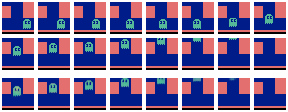
\includegraphics[width=0.92\linewidth]{figures/pred/pac/blurry/pred-sharp.png}
  \caption{}
  \label{fig:pac-pred-sharp_sample}
\end{subfigure}%
\begin{subfigure}{0.49\textwidth}
  \centering
  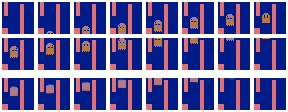
\includegraphics[width=0.92\linewidth]{figures/pred/pac/blurry/pred-blurry.png}
  \caption{}
  \label{fig:pac-pred-blurry_sample}
\end{subfigure}
\caption[Generated MsPacman Patches using Different Loss Functions]{Two predictions showing a similar scene of a moving ghost. The sequence in (a) is predicted using a network trained with the MSE-based triplet loss function, whereas the network in (b) is trained on MAE+GDL loss.} \label{fig:pac-pred-blurry}
\end{figure}


\subsection{Test Results}

Next, we present the test results of our best performing two-layer model. This model is configured as described earlier in this section. In the qualitative assessments, our network takes advantage from the triplet loss function using MSE as its main loss term which produced the most promising results when we explored the behavior of the model on the MsPacman dataset. It is important to note that the test set is not filtering out random crops that show just few or even no movement at all. That's why it is to expect that the average test results can be much better compared to the validation result, since it is quite easy for the network to predict scenes that only contain the maze's static background with no movement at all.


\subsubsection{Quantitative Results}

The image metric results of our network model using the discussed loss function combinations is shown in Table \ref{tab:pac-comparison}. Unfortunately, there is no related project that has published any future frame prediction results on this dataset yet. However, this dataset is indeed used in an independent implementation of \parencite{deep_multiscale_video_pred}. We added the result of some experiments with it for the sake of completion, but these results are hard to compare with ours, because the metrics are calculated on that parts within a frame where motion is actually happening. Additionally, it predicts only one frame given a sequence of four.

As it has been the case on the validation set, the MSE-based triplet loss function produces the best results in all similarity metrics, regardless of it is about the first predicted frame, or the average of the whole future sequence. However, if we look at the sharpness results, the model instance that utilizes no SSIM term in its objective function is able to produce sharper results according to the metric. This is not surprising, because the GDL term is weighted more in this model, which is the central objective of this metric.

\begin{table}[htb]
  \footnotesize
  \centering
  \begin{tabular}{l | r r | r | r r | r}
    \toprule
      \textbf{Loss function} & \multicolumn{3}{c}{\textbf{\nth{1} frame}} & \multicolumn{3}{c}{\textbf{mean of 8 frames}} \\
      & \multicolumn{2}{c}{\scriptsize{Similarity}} & \scriptsize{Sharpness} & \multicolumn{2}{c}{\scriptsize{Similarity}} & \scriptsize{Sharpness} \\
      & PSNR & $\text{SSIM}_{5}$ & SharpDiff & PSNR & $\text{SSIM}_{5}$ & SharpDiff \\
    \midrule
      Adv+GDL \tiny{\parencite{tf_impl_gan}} & 25.3168 & - & 17.2725 & - & - & - \\
    \midrule
      MAE+GDL & 47.5462 & 0.9854 & 27.0217 & 48.6902 & 0.9817 & 27.8182 \\
      MAE+GDL+SSIM & 44.8974 & 0.9917 & 26.9131 & 44.6555 & 0.9856 & 27.9516 \\
      MSE+GDL & 50.5197 & 0.9893 & \textbf{30.0961} & 50.1164 & 0.9833 & \textbf{29.9851} \\
      MSE+GDL+SSIM & \textbf{50.4655} & \textbf{0.9925} & 28.5023 & \textbf{50.2746} & \textbf{0.9862} & 28.7008 \\
    \bottomrule
  \end{tabular}
  \caption[Metric Results on MsPacman]{Metric results of produced patch sequences using a 2-layer model on MsPacman's test split. The achieved similarity and sharpness of the same models using different loss layers are given for both the first frame only and the average of the whole generated future sequence. The results of the other approach in the first row are not comparable to ours due to a different evaluation procedure.}\label{tab:pac-comparison}
\end{table}

Another interesting fact is that the differences between the image metric results of the first predicted frame and the average of all predicted frames are very marginal. This might be due to the reason that the bigger part of each patch is just static, noise-free content. Hence, the actual interesting parts of each frame that include motion have only little effect on the metric results. Furthermore, it is surprising that the sharpness metric results of the first predicted frame are slightly worse compared to the metric's mean over the whole predicted sequence. 

On the other side, the pixel-wise absolute and squared error results in Table \ref{tab:pac-comparison2} appear more plausible. Here, the differences between the first frame and the average of the sequence are significantly larger. But one fact remains unchanged: the networks trained on the MSE-based triplet loss function is able to produce the best prediction results. Furthermore, it is interesting to see that both networks that utilize a squared error loss term as their main objective are able to outperform both other model instances regarding the MAE error, despite the fact the other who networks are explicitly optimized for this for this objective. This superiority could be reasoned by the characteristics of the MsPacman dataset.

\begin{table}[htb]
  \footnotesize
  \centering
  \begin{tabular}{l | r r | r r }
    \toprule
      \textbf{Loss function} & \multicolumn{2}{c}{\textbf{\nth{1} frame}} & \multicolumn{2}{c}{\textbf{mean of 8 frames}} \\
      & MAE & MSE & MAE & MSE \\
    \midrule
      MAE+GDL & 0.0033 & 0.0009 & 0.0041 & 0.0018 \\
      MAE+GDL+SSIM & 0.0031 & \textbf{0.0005} & 0.0047 & 0.0015 \\
      MSE+GDL & 0.0025 & 0.0006 & 0.0040 & 0.0016 \\
      MSE+GDL+SSIM & \textbf{0.0023} & \textbf{0.0005} & \textbf{0.0037} & \textbf{0.0014} \\
    \bottomrule
  \end{tabular}
  \caption[Test Errors on MsPacman]{Absolute and squared error test results on MsPacman dataset using varying loss layers in our 2-layer network.}\label{tab:pac-comparison2}
\end{table}


\subsubsection{Qualitative Results}

For a qualitative evaluation of the network, we take a detailed look at some generated future sequences. Starting the clip in Figure \ref{fig:pac-pred-random1}, the motion of the ghost is predicted very precisely. Moreover, the fine details of the ghost's eyes and zigzag mouth are preserved even until the eighth frame. However, the dynamics of the blue and white blinking effect is not continued in the predicted sequence.

\begin{figure}[h!tb]
\centering
\begin{subfigure}{0.49\textwidth}
  \centering
  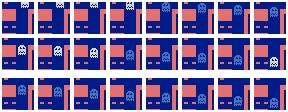
\includegraphics[width=0.92\linewidth]{figures/pred/pac/random/pred-00.png}
  \caption{}
  \label{fig:pac-pred-random1}
\end{subfigure}%
\begin{subfigure}{0.49\textwidth}
  \centering
  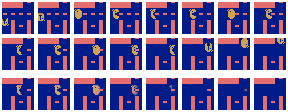
\includegraphics[width=0.92\linewidth]{figures/pred/pac/random/pred-04.png}
  \caption{}
  \label{fig:pac-pred-random2}
\end{subfigure}
\caption[Random Prediction Samples on MsPacman]{Two random prediction samples on MsPacman that contain at least some motion. From top to bottom: ground truth input and output sequence; predicted sequence of the 2-layer network.} \label{fig:pac-pred-random}
\end{figure}

As a second example, the prediction result shown in Figure \ref{fig:pac-pred-random2} is considered. On the one side, pacman's dynamics are correctly continued in first four generated frames. It correctly moves forward, performs chewing and eats the orange dot, but with some delay. On the other side, the game character suddenly disappears when it arrives the second crossing. We observed such a behavior actually quite often in many other samples as well. As a results, this indicates that the network has its issues to decide what direction the moving objects will take within the maze. This assumption can be further confirmed by some other observations, such as that objects reaching a crossing are either affected by a loss of opacity, split up into multiple directions, disappear complete as shown in the demonstrated example, or in best case chose any random direction. Moreover, such disappearance effects take rarely place in corners where there is beside turning around only one other option.

More predictions on small patches can be found in Figure \ref{fig:pac-pred-random_extra} in the appendix. It is worth noting that still-standing motion is particularly well captured and continued by the network. As an example, pacman's chewing animation in Figure \ref{fig:pac-pred-random_extra1} is kept up in all predicted frames, so that it is looks almost identical at the first glance. The only noticeable difference here is that pacman temporarily changes its direction in the fifth frame for just a single time step in the ground truth future.

\begin{figure}[htpb]
	\centering
	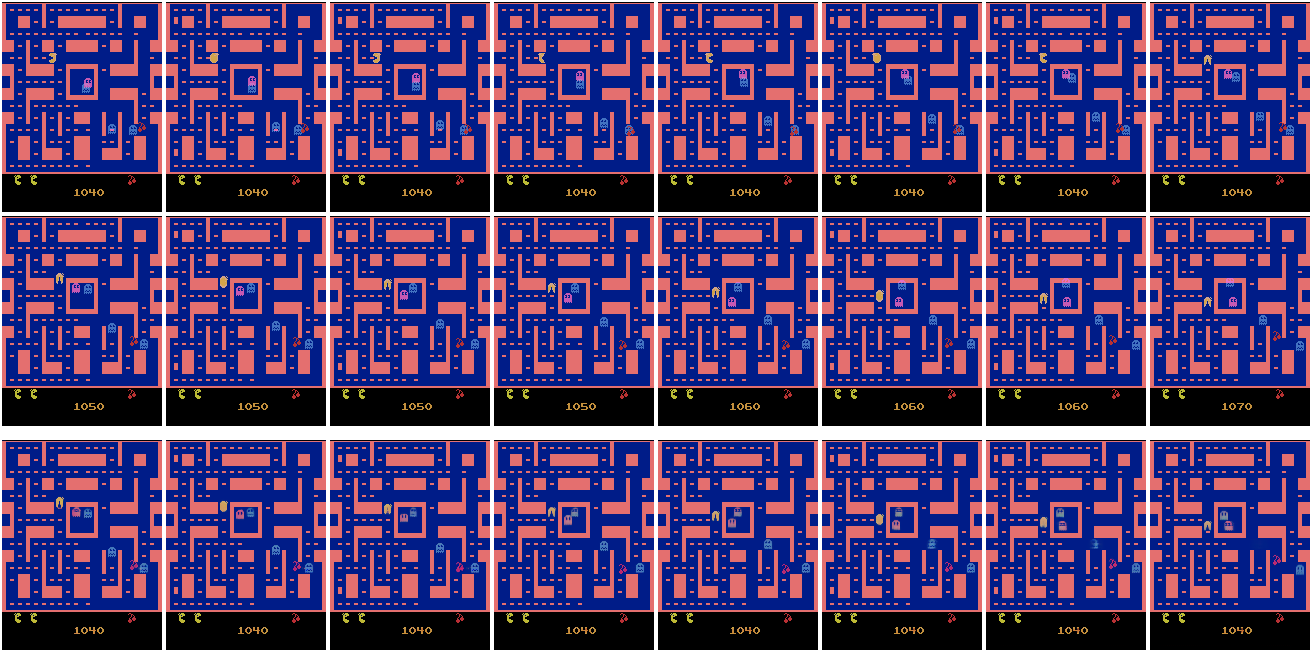
\includegraphics[width=1.0\linewidth]{figures/pred/pac/full/pred-00.png} 
	\caption[Random Full Screen Prediction Sample on MsPacman]{Prediction sample of a full game scene using our 2-layer network, which is trained on small $32 \times 32$ patches only. This is possible due to our FCN approach. From top to bottom: ground truth input and output sequence; predicted game sequence.} \label{fig:pac-pred-full1}
\end{figure}

As explained in section \ref{sec:fcn}, the fully-convolutional approach of our model comes with the advantage that it can be applied on input images of larger size. Therefore, a prediction sample of a sequence showing a full game scene is presented in Figure \ref{fig:pac-pred-full1}. It shows that future frames can indeed be forecasted for the full images with acceptable results as well. For instance, the blinking effect of the large dots in the corners of the maze and the trajectory of the red cherry is predicted almost perfectly. Furthermore, the motion of the game characters is continued quite well, with the exception one ghost that disappears or that both ghosts in the center slightly change their color. A second result showing the full maze can be found in Figure \ref{fig:pac-pred-full2}. in that sample, attention should be paid to the blue ghost in the center, who is correctly predicted to leave the cave instead of going for another spin.

Finally, the stability of the generated future frames investigated by performing predictions on longer sequences. As it can be seen in Figure \ref{fig:pac-pred-full-long}, some artifacts become visible starting from the \nth{14} forecasted frame. And while all moving game characters gradually disappear, the red cherry object is predicted very precisely until the end of the lengthened sequence.













\section{Experiments on UCF-101}

The last experiment investigates the performance of the proposed neural network model on natural videos. More precisely speaking, various network instances are trained on $32 \times 32$ patches from the UCF-101 dataset, which is further described in Section \ref{sec:ds_ucf}. Due to the fact that clips from this dataset show natural scenes with a lot of movement and noise, it can be expected that the inclusion of perceptual motivated bias terms in the loss function is finally able to unfold its full effect. For that reason, the examination of different loss function combinations from the second experiment on MsPacman is repeated for this dataset in the hope that it reveals more significant improvements.

\subsection{Hyperparameter Tuning}

The search for good hyperparameters and the resulting settings are very similar to the outcomes of Section \ref{sec:hyper_pac}. We train several model instances with varying learning rates, but limit the regularization coefficients to a smaller search space in order to save time, in particular $\lambda = \{1e^{-6}, 1e^{-5}\}$. Further, we do not test any single-layer ConvLSTM configuration, argued by the insights of both other experiments. In detail, we perform most trials on two-layer set-ups, and finally use the same configuration using a three-layer ConvLSTM. Even though MSE as the main objective term of the triplet loss function has shown to deliver the best results on MsPacman, we start with the absolute error as the main error term nevertheless. This is due to its positive results in context of natural images, as already mentioned in Section \ref{sec:img-sim-naive} and Chapter \ref{chapter:relatedwork}.

The grid-search ends up with the same model configuration as in the last experiment. But this time, the differences between using different initial learning rates become more noticeable, with lower learning rates in the advantage. Hence, the following investigations are based on an exponential decaying learning rate starting from $\eta = 0.0005$ with a weight decay of $\lambda = 1e^{-5}$. 


\subsubsection*{Loss Layer}

The absolute and squared pixel-wise prediction errors on the validation set using various network configurations are illustrated in Figure \ref{fig:plot-ucf-loss}. It can be clearly seen that the use of MSE produces less accurate predictions compared to all other loss function combinations. While the results of all other configurations are very close together, the error of the MAE-based triplet loss function is slightly in advantage. Even that the diagram presents its results of the trained three-layer network instance, the same is true for the two-layer version.

\begin{figure}[htb]
\centering
\begin{subfigure}{0.5\textwidth}
  \centering
  \pgfplotstableset{col sep=comma}
  \pgfplotstableread{data/ucf/loss/mse/run_ucf-ss-3l3i5hp-c326464k533s121bn-wd1e-05-mae-triplet-DQ_validation_mse.csv}\modelA
  \pgfplotstableread{data/ucf/loss/mse/run_ucf-ss-2l3i5hp-c326464k533s121bn-wd1e-05-mae-triplet-LB_validation_mse.csv}\modelB
  \pgfplotstableread{data/ucf/loss/mse/run_ucf-ss-2l3i5hp-c326464k533s121bn-wd1e-05-mae-noGDL-IF_validation_mse.csv}\modelC
  \pgfplotstableread{data/ucf/loss/mse/run_ucf-ss-2l3i5hp-c326496k533s122bn-wd1e-05-mae-VN_validation_mse.csv}\modelD
  \pgfplotstableread{data/ucf/loss/mse/run_ucf-ss-2l3i5hp-c326464k533s121bn-wd1e-05-mse-IZ_validation_mse.csv}\modelE
  \hspace*{-0.6cm}
  {
  \begin{tikzpicture}[scale=0.5]
    \begin{axis}[
        ymode=log,
    	log ticks with fixed point,
        xmin=0,
        xmax=65000,
        ytick={0.01,0.02,0.05,0.1},
        legend style={legend pos=north east},
        grid,
        thick,
        ylabel=MSE loss,
        xlabel=step \textit{i},
        x post scale=1.6,
      ]
      \addplot[draw=black!30!violet] table[x=Step, y=Value]{\modelE};
      \addlegendentry{MSE+GDL (valid)};
      \addplot[draw=black!30!orange] table[x=Step, y=Value]{\modelC};
      \addlegendentry{MAE (valid)};
      \addplot[draw=black!30!red] table[x=Step, y=Value]{\modelD};
      \addlegendentry{MAE+GDL 96filters (valid)};
      \addplot[draw=black!30!blue] table[x=Step, y=Value]{\modelB};
      \addlegendentry{MAE+GDL+SSIM (valid)};
      %best
      \addplot[draw=black!30!green] table[x=Step, y=Value]{\modelA};
      \addlegendentry{MAE+GDL+SSIM 3layers (valid)};
    \end{axis}
  \end{tikzpicture}
  }
  \caption{}
  \label{fig:plot-ucf-loss-mse}
\end{subfigure}%
\begin{subfigure}{0.5\textwidth}
  \centering
  \pgfplotstableset{col sep=comma}
  \pgfplotstableread{data/ucf/loss/mae/run_ucf-ss-3l3i5hp-c326464k533s121bn-wd1e-05-mae-triplet-DQ_validation_mae.csv}\modelA
  \pgfplotstableread{data/ucf/loss/mae/run_ucf-ss-2l3i5hp-c326464k533s121bn-wd1e-05-mae-triplet-LB_validation_mae.csv}\modelB
  \pgfplotstableread{data/ucf/loss/mae/run_ucf-ss-2l3i5hp-c326464k533s121bn-wd1e-05-mae-noGDL-IF_validation_mae.csv}\modelC
  \pgfplotstableread{data/ucf/loss/mae/run_ucf-ss-2l3i5hp-c326496k533s122bn-wd1e-05-mae-VN_validation_mae.csv}\modelD
  \pgfplotstableread{data/ucf/loss/mae/run_ucf-ss-2l3i5hp-c326464k533s121bn-wd1e-05-mse-IZ_validation_mae.csv}\modelE
  \hspace*{-0.6cm}
  {
  \begin{tikzpicture}[scale=0.5]
    \begin{axis}[
        ymode=log,
    	log ticks with fixed point,
        xmin=0,
        xmax=65000,
        ytick={0.08,0.15,0.25},
        legend style={legend pos=north east},
        grid,
        thick,
        ylabel=MAE loss,
        xlabel=step \textit{i},
        x post scale=1.6,
      ]
      \addplot[draw=black!30!violet] table[x=Step, y=Value]{\modelE};
      \addlegendentry{MSE+GDL (valid)};
      \addplot[draw=black!30!orange] table[x=Step, y=Value]{\modelC};
      \addlegendentry{MAE (valid)};
      \addplot[draw=black!30!red] table[x=Step, y=Value]{\modelD};
      \addlegendentry{MAE+GDL 96filters (valid)};
      \addplot[draw=black!30!blue] table[x=Step, y=Value]{\modelB};
      \addlegendentry{MAE+GDL+SSIM (valid)};
      %best
      \addplot[draw=black!30!green] table[x=Step, y=Value]{\modelA};
      \addlegendentry{MAE+GDL+SSIM 3-layers (valid)};
    \end{axis}
  \end{tikzpicture}
  }
  \caption{}
  \label{fig:plot-ucf-loss-mae}
\end{subfigure}
\caption[Comparison of Losses on UCF-101]{Comparison of validation results on UCF-101 using similar network configurations with varying loss functions. All models have been trained given an input sequence of 10 patches of size $32 \times 32$ to predict the next 10 frames. The loss values shown represent the per-pixel error. All models except one are using the vanilla configuration with 64 filters within the ConvLSTM cells.} \label{fig:plot-ucf-loss}
\end{figure}

The advantages of a network which is trained using the triplet loss function become more visible when the differences in sharpness are considered. At least the sharpness metric in Figure \ref{fig:plot-ucf-loss-sdiff} quantifies such a hypothesis.



\begin{figure}[htb]
\centering
\begin{subfigure}{0.5\textwidth}
  \centering
  \pgfplotstableset{col sep=comma}
  \pgfplotstableread{data/ucf/loss/sdiff/run_ucf-ss-3l3i5hp-c326464k533s121bn-wd1e-05-mae-triplet-DQ_validation_sharpdiff.csv}\modelA
  \pgfplotstableread{data/ucf/loss/sdiff/run_ucf-ss-2l3i5hp-c326464k533s121bn-wd1e-05-mae-triplet-LB_validation_sharpdiff.csv}\modelB
  \pgfplotstableread{data/ucf/loss/sdiff/run_ucf-ss-2l3i5hp-c326464k533s121bn-wd1e-05-mae-noGDL-IF_validation_sharpdiff.csv}\modelC
  \pgfplotstableread{data/ucf/loss/sdiff/run_ucf-ss-2l3i5hp-c326496k533s122bn-wd1e-05-mae-VN_validation_sharpdiff.csv}\modelD
  \hspace*{-0.6cm}
  {
  \begin{tikzpicture}[scale=0.5]
    \begin{axis}[
    	log ticks with fixed point,
        ymin=10,
        ymax=15,
        xmin=0,
        xmax=65000,
        legend style={legend pos=south east},
        grid,
        thick,
        ylabel=SharpDiff,
        xlabel=step \textit{i},
        x post scale=1.6,
      ]
      \addplot[draw=black!30!orange] table[x=Step, y=Value]{\modelC};
      \addlegendentry{MAE (valid)};
      \addplot[draw=black!30!red] table[x=Step, y=Value]{\modelD};
      \addlegendentry{MAE+GDL 96filters (valid)};
      \addplot[draw=black!30!blue] table[x=Step, y=Value]{\modelB};
      \addlegendentry{MAE+GDL+SSIM (valid)};
      %best
      \addplot[draw=black!30!green] table[x=Step, y=Value]{\modelA};
      \addlegendentry{MAE+GDL+SSIM 3-layers (valid)};
    \end{axis}
  \end{tikzpicture}
  }
  \caption{}
  \label{fig:plot-ucf-loss-sdiff}
\end{subfigure}%
\begin{subfigure}{0.5\textwidth}
  \centering
  \pgfplotstableset{col sep=comma}
  \pgfplotstableread{data/ucf/loss/ssim/run_ucf-ss-3l3i5hp-c326464k533s121bn-wd1e-05-mae-triplet-DQ_validation_ssim5.csv}\modelA
  \pgfplotstableread{data/ucf/loss/ssim/run_ucf-ss-2l3i5hp-c326464k533s121bn-wd1e-05-mae-triplet-LB_validation_ssim5.csv}\modelB
  \pgfplotstableread{data/ucf/loss/ssim/run_ucf-ss-2l3i5hp-c326464k533s121bn-wd1e-05-mae-noGDL-IF_validation_ssim5.csv}\modelC
  \pgfplotstableread{data/ucf/loss/ssim/run_ucf-ss-2l3i5hp-c326496k533s122bn-wd1e-05-mae-VN_validation_ssim5.csv}\modelD
  \hspace*{-0.6cm}
  {
  \begin{tikzpicture}[scale=0.5]
    \begin{axis}[
    	log ticks with fixed point,
        ymin=0.5,
        ymax=0.7,
        xmin=0,
        xmax=65000,
        legend style={legend pos=south east},
        grid,
        thick,
        ylabel=SSIM,
        xlabel=step \textit{i},
        x post scale=1.6,
      ]
      \addplot[draw=black!30!orange] table[x=Step, y=Value]{\modelC};
      \addlegendentry{MAE (valid)};
      \addplot[draw=black!30!red] table[x=Step, y=Value]{\modelD};
      \addlegendentry{MAE+GDL 96filters (valid)};
      \addplot[draw=black!30!blue] table[x=Step, y=Value]{\modelB};
      \addlegendentry{MAE+GDL+SSIM (valid)};
      %best
      \addplot[draw=black!30!green] table[x=Step, y=Value]{\modelA};
      \addlegendentry{MAE+GDL+SSIM 3-layers (valid)};
    \end{axis}
  \end{tikzpicture}
  }
  \caption{}
  \label{fig:plot-ucf-loss-ssim}
\end{subfigure}
\caption[Comparison of Image Metrics on UCF-101]{Computed image metrics computed on the UCF-101 dataset. All four networks use the same hyperparameter settings, but differ in the number of recurrent layers, as well as the used objective function.} \label{fig:plot-ucf-imgmetric}
\end{figure}








\subsection{Test Results}

In the following, the test results of different network configurations are presented in a quantitative and qualitative analysis. Like in the previous experiments on MsPacman, it is worth mentioning that the video patches from the test set are not filtered in case they show very less movement.

\subsubsection{Quantitative Results}

Starting with the qualitative test results, Table \ref{tab:ucf-comparison} compares several configurations of our model with outcomes from related works on various image similarity or sharpness metrics. It demonstrates test results of the first predicted frame, as well as the average metric values of the forecasted 10 frames long sequence. However, the results of our model are not really comparable with \parencite{deep_multiscale_video_pred}, since they calculate the metrics on specific regions of the image, where the optical flow exceeds a specified threshold.

\begin{table}[htb]
  \footnotesize
  \centering
  \begin{tabular}{l | r r | r | r r | r}
    \toprule
      \textbf{Loss function} & \multicolumn{3}{c}{\textbf{\nth{1} frame}} & \multicolumn{3}{c}{\textbf{mean of 10 frames}} \\
      & \multicolumn{2}{c}{\scriptsize{Similarity}} & \scriptsize{Sharpness} & \multicolumn{2}{c}{\scriptsize{Similarity}} & \scriptsize{Sharpness} \\
      & PSNR & SSIM & & PSNR & SSIM & \\
    \midrule
      single-scale $\ell_2$ \tiny{\parencite{deep_multiscale_video_pred}} & 26.5 & 0.84 & 24.7 & - & - & - \\
      multi-scale $\ell_1$ \tiny{\parencite{deep_multiscale_video_pred}} & 28.7 & 0.88 & 24.8 & - & - & - \\
      multi-scale GDL+$\ell_1$ \tiny{\parencite{deep_multiscale_video_pred}} & 29.4 & 0.90 & 25.0 & - & - & - \\
      multi-scale Adv+GDL \tiny{\parencite{deep_multiscale_video_pred}} & 31.5 & 0.91 & 25.4 & - & - & - \\
    \midrule
      MSE+GDL & 15.9652 & 0.7112 & 13.6947 & 22.5218 & 0.7016 & 14.5219 \\
      MAE & 30.8241 & 0.9043 & 17.0282 & 25.9873 & 0.7653 & 15.4952 \\
      $\text{MAE+GDL}_{96}$ & 29.4092 & \textbf{0.9047} & 16.7509 & 25.8577 & 0.7686 & 15.4089 \\
      MAE+GDL+SSIM & \textbf{31.3144} & 0.7668 & \textbf{17.3785} & \textbf{26.6385} & 0.7668 & 15.7363 \\
      MAE+GDL+SSIM 3layers & 29.4000 & 0.9031 & 17.2316 & 26.2130 & 0.7679 & \textbf{15.7283} \\
    \bottomrule
  \end{tabular}
  \caption[Metric Results on UCF-101]{Metric results of predicted patch sequences using our approach on the UCF-101 test split. The achieved similarity and sharpness results by using different loss layers are given for both the first frame only and the mean of the generated sequence. All our models are trained for the same amount of time, in detail the 2-layer networks for \num{100000} and the 2-layer network for \num{68000} iterations. The results of both listed approaches are not comparable, because the other one takes only the moving areas of the images into account.}\label{tab:ucf-comparison}
\end{table}

When we take a look at the achieved test results listed in Table \ref{tab:ucf-comparison}, it can be seen that the use of absolute error as the main objective function produces much better results in all cases in comparison to squared error. These same fact has already been observed during the search for the optimal hyperparameters of the model. But it might be doubted that the metric results of the first predicted frame using the MSE+GDL loss are actually worse compared to the mean of the entire forecasted sequence. However, a quick look at Figure \ref{fig:ucf-comparison} (row 15, columns 1) indicates that this network indeed has its issues with the brightness of the first generated image.

While the use of the third recurrent layer does not seem to be from advantage, it has to be noted that this network is trained for fewer iterations. Thus, the results represent different networks that are trained for roughly the same amount of time. Although the two-layer network using the triplet loss function is slightly outperforming the other models, its SSIM index result is far beyond all three other MAE-based networks.

\subsubsection{Qualitative Results}

For a qualitative evaluation of the model, many prediction results have been analyzed regarding the perceptual similarity to the ground truth future. Two selected sequences are therefore depicted in Figure \ref{fig:ucf-random1}. Both predictions are visibly affected by a blur effect the further the network has to look into the future. Nevertheless, a slight notion of movement is noticeable at the beginning of all presented clips. Especially the swimmer in Figure \ref{fig:ucf-random1b} is continued quite precisely, although he enters the scene just at the very end if the input sequence. Further examples of predicted patches can be found in Figure \ref{fig:ucf-random2} in the appendix.

\begin{figure}[h!tb]
\centering
\begin{subfigure}{0.49\textwidth}
  \centering
  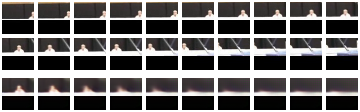
\includegraphics[width=0.92\linewidth]{figures/pred/ucf/random/pred-00.png}
  \caption{}
  \label{fig:ucf-random1a}
  \vspace{.1cm}
\end{subfigure}
\begin{subfigure}{0.49\textwidth}
  \centering
  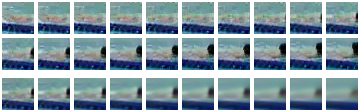
\includegraphics[width=0.92\linewidth]{figures/pred/ucf/random/pred-04.png}
  \caption{}
  \label{fig:ucf-random1b}
  \vspace{.1cm}
\end{subfigure}
\caption[Prediction Samples on UCF-101]{Two prediction examples using our 2-layer ConvLSTM model. From top to bottom: Input and ground truth frames; prediction results.}
\label{fig:ucf-random1}
\end{figure}

Fortunately, the UCF-101 dataset has been applied in many related studies as well. It is therefore possible to do a more extensive comparison with outcomes of different approaches. Results from an FC-LSTM encoder-decoder network, different convolutional with or without adversarial training and various combinations of loss functions are collected in Figure \ref{fig:ucf-comparison}. When comparing the predicted sequences of non-adversarial networks with the results of our models in the last group at the bottom of the graphic, it can be seen that their outcomes are generally blurrier. However, a clear motion is also not discernible in the forecasted frames of our model. Although the predictions of the adversarial networks do not look close to the ground truth on the long term, they indeed remain very realistic.

\begin{figure}[htpb]
	\centering
	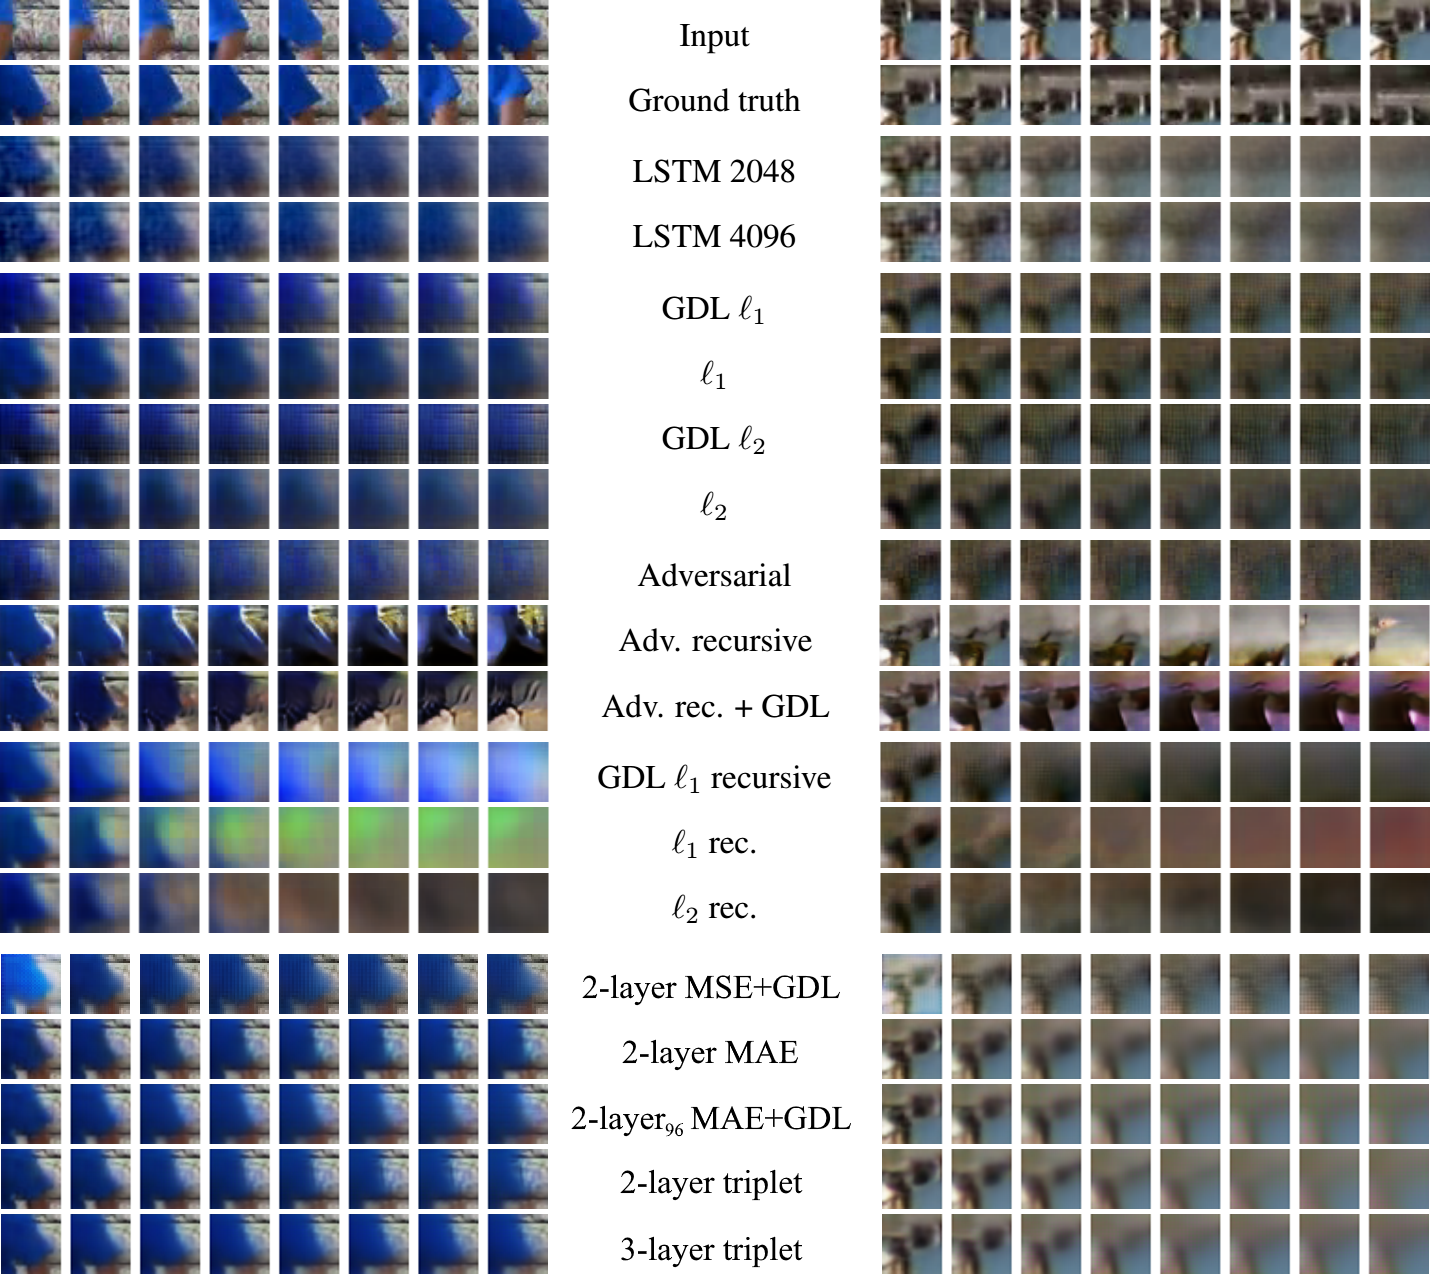
\includegraphics[width=1.0\linewidth]{figures/pred/ucf/ucf_compare.png} 
	\caption[Qualitative Comparison to Competing Models]{Qualitative comparison to different approaches, including various objective functions. From top to bottom: input and ground truth target frames; FC-LSTM results; simple encoder-decoder CNN that predicts 8 future frames given 8 input patches; the same CNN but with adversarial training; simple encoder-decoder CNN that recursively predicts a single frame give 4 patches; our model in its vanilla configuration, except $\text{2-layer}_{96}$ where 96 feature maps are used in each ConvLSTM cell. (Based on \parencite[p. 13]{deep_multiscale_video_pred})} \label{fig:ucf-comparison}
\end{figure}

Additional Long-term predictions are also performed in order to assess the networks stability regarding its predictions. One example sequence, in which the network predicts twice as many frames as it has been trained for, is demonstrated in Figure \ref{fig:ucf-long1}. When we consider the consider the whole sequence from the first until the very last frame, a tendency of the head to move slowly downwards can indeed be observed. However, the predictions are getting more and more burry as expected. For a second long-term example of a soccer player, see Figure \ref{fig:ucf-long2} in the appendix. It reveals that the network has its issues to predict the accurate future of small or thin details of the content that move quite fast. In this case, the player's legs tend to vanish until the end of the sequence. The swift disappearance of fast moving object can be observed in many other examples as well. As a consequence, this might indicate that the used hidden-to-hidden kernel size of $5 \times 5$ within the ConvLSTM cells, or the kernels of the other convolutional layers, is too small to capture such motion. 

\begin{figure}[htpb]
	\centering
	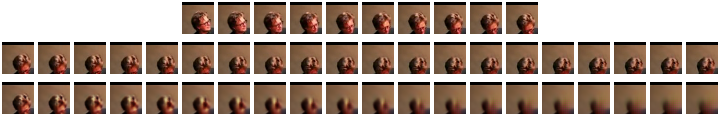
\includegraphics[width=1.0\linewidth]{figures/pred/ucf/long/pred-01.png} 
	\caption[Out-of-Domain Prediction Samples on UCF-101]{Two out-of-domain prediction examples where the network predicted 20 patches, while being trained to predict only 10 frames. From top to bottom: Input and ground truth frames; prediction results from our 2-layer ConvLSTM model.} \label{fig:ucf-long1}
\end{figure}

Finally, the probably most interesting test scenario is investigated: future frame predictions using the full-size video frames. Two examples concerning this matter are depicted in Figure \ref{fig:ucf-full1}, but more examples can be found in the appendix in Figure \ref{fig:ucf-full2}. We can see that the quality of results is similar to the previous scenarios. In almost every sample, static background is predicted very precisely. Even fine detail of the background can be preserved until the end of the predicted sequence, such as the wall's tile pattern in Figure \ref{fig:ucf-full1a}. Furthermore, some few examples are able to capture more complex dynamics of the scene. For instance, forecasting the skier's loping position in Figure \ref{fig:ucf-full1b}.

\begin{figure}[h!tb]
\centering
\begin{subfigure}{1.0\textwidth}
  \centering
  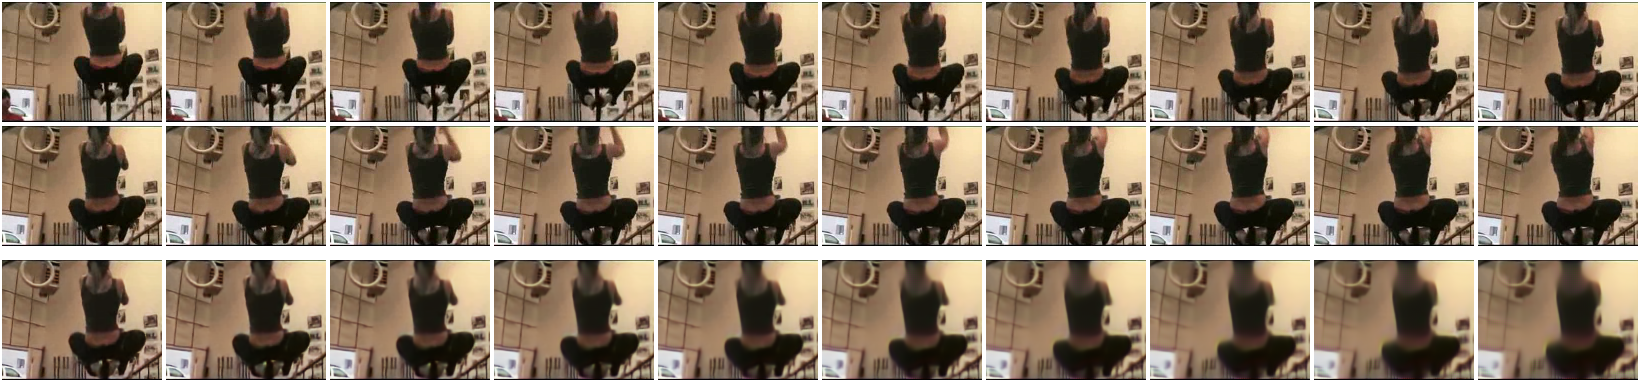
\includegraphics[width=1.0\linewidth]{figures/pred/ucf/full/pred-00.png}
  \caption{}
  \label{fig:ucf-full1a}
  \vspace{.1cm}
\end{subfigure}
\begin{subfigure}{1.0\textwidth}
  \centering
  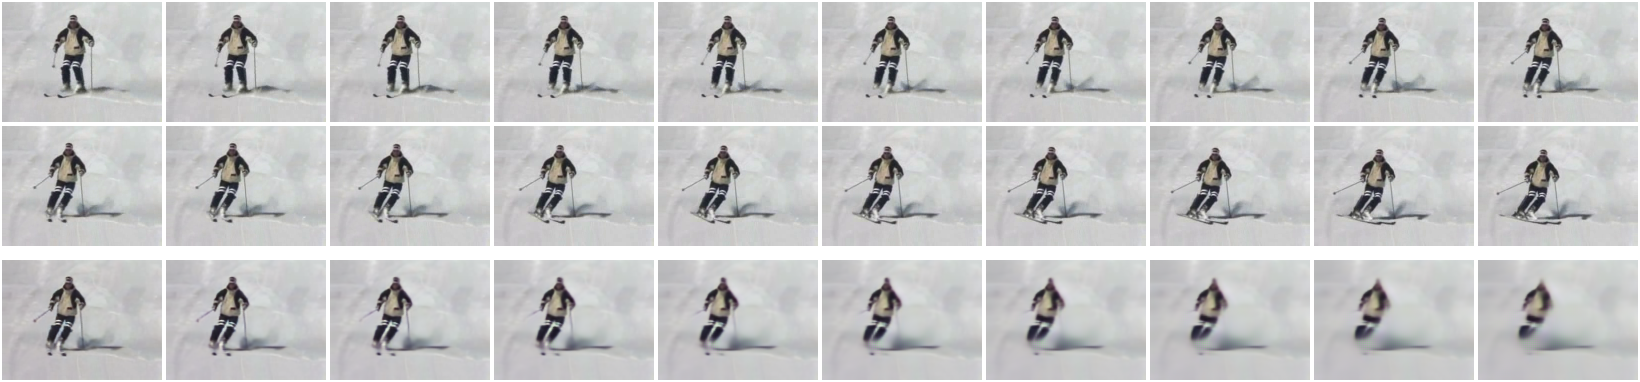
\includegraphics[width=1.0\linewidth]{figures/pred/ucf/full/pred-01.png}
  \caption{}
  \label{fig:ucf-full1b}
  \vspace{.1cm}
\end{subfigure}
\caption[Full Frame Prediction Sample on UCF-101]{Prediction samples of full video frames, enabled due to our fully-convolutional approach. These have been generated using a 2-layer network that is trained on smaller $32 \times 32$ patches. From top to bottom: ground truth input and output sequence; predicted future of the video.}
\label{fig:ucf-full1}
\end{figure}
